%********************************************************************************************
%								COMANDOS ÚTILES PARA LATEX EN ESTE TP							
%
%	\ : espacio simple
%	\\ : nueva línea
%	\par : va a la línea de abajo y deja sangría
%	\vspace{##tamaño en pt##} o \vspace{\baselineskip} en general:
%								 para dejar un espacio vertical
%	\textbf{text} :text en negrita
%	\textit{text} :text en itálica
%
% GRAFICOS CENTRADOS:
%	\begin{center}
%		\includegraphics[width=\textwidth]{./img/##ruta imagen (no hace falta extension)##}
%	\end{center}
%		--> se pueden agregar atributos como scale por si se hace muy grande
%
% TABLAS CENTRADAS:
%	\begin{center}
%	\begin{tabular}{|c|c|}
%	\hline
%	\ \textbf{Programa} & \textbf{Ticks} \\
%	\hline
%		ASM & 675127609 \\
%	\hline
%	\end{tabular}
%	\end{center}
%
% ALGORITMOS (EN VARIOS LENGUAJES):
% \begin{lstlisting}
%	void sumoDiez(int &num)
%	{
%	    num += 10;
%	}
%	
%	int main()
%	{
% 	   int i;
%	    int numeroAProcesar = 20;
%	    for (i = 0; i < 50; i++)
%	    {
%	        sumoDiez(numeroAProcesar);	//Proceso el numero en cada ciclo
%	    } 
%	    return 0;
%	}
%	\end{lstlisting}
%
% para info sobre todo lo que tiene el package detallado:
% http://en.wikibooks.org/wiki/LaTeX/Source\_Code\_Listings
%
%********************************************************************************************

\documentclass[10pt,a4paper]{article}
\usepackage[utf8]{inputenc} % para poder usar tildes en archivos UTF-8
\usepackage[spanish]{babel} % para que comandos como \today den el resultado en castellano
\usepackage{a4wide} % márgenes un poco más anchos que lo usual
\usepackage[conEntregas]{caratula}
\usepackage{amssymb}
\usepackage{fancybox}
\usepackage[usenames,dvipsnames]{color}
\usepackage{hyperref}
\usepackage{listings}
\usepackage{xcolor}
\usepackage{amsmath}

\hypersetup{
    colorlinks,
    citecolor=black,
    filecolor=black,
    linkcolor=black,
    urlcolor=black
}

\lstdefinestyle{customc}{
  belowcaptionskip=1\baselineskip,
  breaklines=true,
  frame=L,
  xleftmargin=\parindent,
  language=C,
  showstringspaces=false,
  basicstyle=\footnotesize\ttfamily,
  keywordstyle=\bfseries\color{green!40!black},
  commentstyle=\itshape\color{purple!40!black},
  identifierstyle=\color{blue},
  stringstyle=\color{orange},
}

\lstset{escapechar=@,style=customc}

\begin{document}

\titulo{Trabajo Práctico 1}
\subtitulo{Wiretapping}

\fecha{\today}

\materia{Teoría de las Comunicaciones}
\grupo{}

\integrante{Barbeito, Nicolás}{LLL/AA}{nicolasbarbeiton@gmail.com}
\integrante{Garassino, Agustín Javier}{394/12}{ajgarassino@gmail.com}
\integrante{Vileriño, Silvio}{LLL/AA}{svilerino@gmail.com}

\maketitle

\tableofcontents
\newpage

\section{Introducción}
El objetivo de este trabajo es construir una herramienta para el análisis de redes, más específicamente de la interacción de sus miembros a través de paquetes ARP (Address Resolution Protocol). Posteriormente, esta se utilizará como medio para la realización de experimentos en diversos entornos y sacar conclusiones a partir de los datos recolectados. Es decir, se recopilárá información sobre distintas redes y se tratará de deducir información significante para cada una de ellas a partir de su tráfico de paquetes ARP.

\section{Herramienta para análisis de la red}
\subsection{Paquetes ARP}
Hoy en día la mayoría de los dispositivos con acceso a la red poseen al menos dos direcciones asociadas que permiten identificarlo unívocamente y diferenciarlo del resto. La primera de ellas, denominada MAC Address o dirección física, consiste en un identificador de 6 bytes. Esta es utilizada por diversas tecnologías de capa 2 según el modelo OSI \footnote{Modelo OSI: http://www.ecma-international.org/activities/Communications/TG11/s020269e.pdf}, por ejemplo en ethernet\footnote{Ethernet: IEEE 802.3} o las redes inalámbricas\footnote{Wi-Fi: IEEE 802.11}. La segunda es llamada dirección IP: está formada por 4 bytes y opera en la capa 3 del modelo OSI. Como estas direcciones operan a distintas capas del modelo necesitan un protocolo auxiliar que asocie las direcciones de ambos tipos a una misma máquina.

\vspace{\baselineskip}
        \begin{center}
        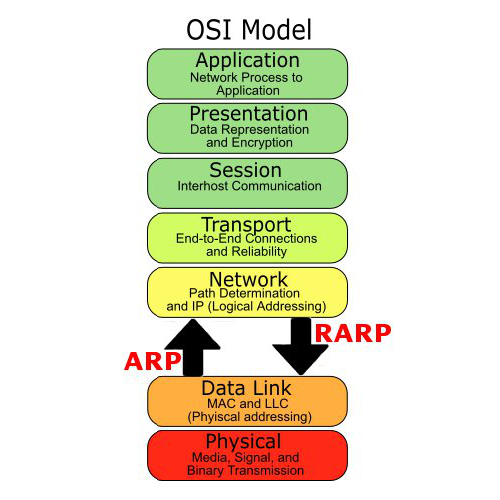
\includegraphics[scale=0.40]{osimodel.jpeg}
        \\
        \vspace{1pt}
        \footnotesize\textit{Modelo OSI. Se puede ver como el protocolo ARP se encarga de la comunicación entre la capa 2 y la capa 3.}
      \end{center}
    \vspace{\baselineskip}
\par

Es decir que el protocolo ARP surge por la necesidad de una máquina de comunicarse con otra en su misma red utilizando una tecnología de la capa nivel 2, teniendo en su poder una dirección de nivel 3. Para cumplir con su objetivo, el protocolo ARP provee dos operaciones:

\begin{itemize}
\item \textit{who-has}: La máquina manda una señal broadcast (paquete que reciben todas las computadoras en la red) preguntando quién posee una dirección IP determinada, con el fin de obtener la MAC Address asociada.
\item \textit{reply}: Cuando la máquina recibe un paquete ARP \textit{who-has} preguntando por su dirección, contesta únicamente al dispositivo de donde provino avisando cuál es su MAC Address.
\end{itemize}

Además cada una de las máquinas posee una tabla asociando direcciones MAC con IP de los dispositivos en la red. El propósito de esta tabla es reducir el tráfico de paquetes ARP, utilizando las operaciones solo cuando sea necesario actualizar la tabla.

\subsection{Implementación y uso}
La herramienta para el análisis de la red fue desarrollada en el lenguaje de programación Python, con la ayuda de diversas librerías que proveen herramientas para la manipulación de paquetes en la red \footnote{Scapy: http://www.secdev.org/projects/scapy/} y generación de visualizaciones amigables de los datos recopilados. Una vez ejecutado, el programa se encarga de filtrar los paquetes ARP que detecte en la red y obtener datos estadísticos a partir de estos. Entre otras cosas, calcula la entropía considerando a las direcciones IP destino u origen de los paquetes como una fuente de información.

\section{Experimentación}
Para facilitar la lectura de ambos tipos de direcciones a los humanos, generalmente las primeras son escritas como números hexadecimales separados por ':', mientras que las direcciones IP se escriben como números decimales separados por puntos. Siendo, por ejemplo, 00:22:b0:00:f2:61 una MAC Address válida y 192.168.1.10 una dirección IP.

\section{Conclusiones}

\end{document}